\documentclass{report}

\title{Solving Rubik's Cube with Lego Mindstorms}
\date{03-05-2018}
\author{Will Garside}

\usepackage[a4paper,left=2.54cm,right=2.54cm, top=2.54cm, bottom=2.54cm]{geometry}	% better margins
\usepackage{booktabs} 			% tables with nice formatting
\usepackage{tabularx}			% tables with proper width
\usepackage{multirow}			% multi-row cells in table
\usepackage{gensymb}			% symbols
\usepackage[british]{babel}		% sets language formatting to British
\usepackage{csquotes}			% quoting commands
\usepackage[table]{xcolor}		% font colouring / table cell colouring
\usepackage{epigraph}			% epigraphs in chapters
\usepackage{parskip}			% better paragraph formatting
\usepackage{graphicx}			% image package
\usepackage{longtable} 			% To display tables on several pages
\usepackage{pgfgantt}			% Gantt Charts
\usepackage{pgfplots}			% draw charts and graphs
\usepackage{titlesec}			% used in chapter titles
\usepackage{subcaption}			% allows sub-figures
\usepackage{algorithm}			% algorithms
\usepackage{algpseudocode}		% algorithm formatting
\usepackage[fleqn]{amsmath}		% multiline math
\usepackage{amssymb}			% math symbols
\usepackage{xparse}				% adds string substitution for moveset command
\usepackage{courier}			% adds inline Courier font
\usepackage{siunitx}			% SI unit support
\usepackage{listings}			% code formatting
\usepackage{enumitem}			% Lettered enumerations

\titleformat{\chapter}{\normalfont\Huge\bfseries}{\thechapter}{1em}{}
\titlespacing*{\chapter}{0pt}{3.5ex plus 1ex minus .2ex}{2.3ex plus .2ex}

\usepgfplotslibrary{dateplot}	% use date in pgfplot
\pgfplotsset{compat=1.8}

\lstset{ 
%	backgroundcolor=\color{white},   % choose the background color; you must add \usepackage{color} or \usepackage{xcolor}; should come as last argument
	basicstyle=\small\ttfamily,        % the size of the fonts that are used for the code
%	breakatwhitespace=false,         % sets if automatic breaks should only happen at whitespace
%	breaklines=true,                 % sets automatic line breaking
%	captionpos=b,                    % sets the caption-position to bottom
	commentstyle=\color{mygreen},    % comment style
%	deletekeywords={...},            % if you want to delete keywords from the given language
%	escapeinside={\%*}{*)},          % if you want to add LaTeX within your code
%	extendedchars=true,              % lets you use non-ASCII characters; for 8-bits encodings only, does not work with UTF-8
%	frame=single,	                   % adds a frame around the code
	keepspaces=true,                 % keeps spaces in text, useful for keeping indentation of code (possibly needs columns=flexible)
	keywordstyle=\color{blue},       % keyword style
	language=Python,                 % the language of the code
%	morekeywords={*,...},            % if you want to add more keywords to the set
%	numbers=left,                    % where to put the line-numbers; possible values are (none, left, right)
%	numbersep=5pt,                   % how far the line-numbers are from the code
%	numberstyle=\tiny\color{mygray}, % the style that is used for the line-numbers
%	rulecolor=\color{black},         % if not set, the frame-color may be changed on line-breaks within not-black text (e.g. comments (green here))
%	showspaces=false,                % show spaces everywhere adding particular underscores; it overrides 'showstringspaces'
%	showstringspaces=false,          % underline spaces within strings only
%	showtabs=false,                  % show tabs within strings adding particular underscores
%	stepnumber=2,                    % the step between two line-numbers. If it's 1, each line will be numbered
%	stringstyle=\color{mymauve},     % string literal style
%	tabsize=2,	                   % sets default tabsize to 2 spaces
%	title=\lstname                   % show the filename of files included with \lstinputlisting; also try caption instead of title
}

\newcolumntype{M}[1]{>{\centering\arraybackslash}m{#1}}
\newcommand{\tbo}[1]{\textbf{#1}}
\newcommand{\tit}[1]{\textit{#1}}
\newcommand{\tun}[1]{\underline{#1}}
\newcommand{\propernoun}[1]{\enquote{\tit{#1}}}
\newcommand{\legopiece}[1]{(\#\tbo{#1})}
\newcommand{\moveset}[1]{\uppercase{\texttt{\{\formatmoves{#1}\}}}}
\newcommand{\movesequence}[1]{\uppercase{\texttt{:\formatmoves{#1}:}}}
\newcommand{\movegroup}[1]{\uppercase{\texttt{\formatmoves{#1}}}}
\newcommand{\face}[1]{\uppercase{\texttt{\formatmovesnospace{#1}}}-face}
\newcommand{\move}[1]{\uppercase{\texttt{\formatmovesnospace{#1}}}-move}
\newcommand{\colour}[1]{\uppercase{\tit{\texttt{\formatmoves{#1}}}}}
\newcommand{\slice}[1]{\uppercase{\texttt{\formatmovesnospace{#1}}}-slice}
\newcommand{\uscore}{\texttt{\char`_}}

\ExplSyntaxOn
\NewDocumentCommand{\formatmoves}{m}
{
	\tl_set:Nn \l__maxd_argument_tl { #1 }
	\tl_replace_all:Nnn \l__maxd_argument_tl { ' } { '\; }
	\tl_replace_all:Nnn \l__maxd_argument_tl { . } { \;\; }
	\tl_replace_all:Nnn \l__maxd_argument_tl { ~ } { \; }
	\tl_replace_all:Nnn \l__maxd_argument_tl { 2 } { \textsuperscript{2}\; }
	\tl_use:N \l__maxd_argument_tl
}

\NewDocumentCommand{\formatmovesnospace}{m}
{
	\tl_set:Nn \l__maxd_argument_tl { #1 }
	\tl_replace_all:Nnn \l__maxd_argument_tl { ' } { ' }
	\tl_replace_all:Nnn \l__maxd_argument_tl { . } { \; }
	\tl_replace_all:Nnn \l__maxd_argument_tl { ~ } { \; }
	\tl_replace_all:Nnn \l__maxd_argument_tl { 2 } { \textsuperscript{2} }
	\tl_use:N \l__maxd_argument_tl
}

\tl_new:N \l__maxd_argument_tl
\ExplSyntaxOff

\begin{document}
	\pagenumbering{gobble}
	\maketitle
	\newpage
	
	\renewcommand{\thechapter}{\Roman{chapter}}
	\pagenumbering{roman}
	\chapter{Signed Declaration}
	All sentences or passages quoted in this report from other people's work have been specifically acknowledged by clear cross-referencing to author, work and page(s). Any illustrations which are not the work of the author of this report have been used with the explicit permission of the originator and are specifically acknowledged. I understand that failure to do this amounts to plagiarism and will be considered grounds for failure in this project and the degree examination as a whole.
	\\Name: Will Garside
	\\Signature:
	\\Date: 

	\newpage
	\chapter{Abstract}
	This should be two or three short paragraphs (100-150 words total), summarising the report. A suggested flow is background, project aims, and achievements to date. It should not simply be a restatement of the original project outline
	
	\newpage
	\chapter{Acknowledgements}
	Thanks to my parents, who raised me since I was a boy. And Rik van Grol, who raised me afterwards.
	
	\newpage
	\chapter{Definitions and Notations}
	\addcontentsline{toc}{section}{Basic Definitions}
	\begin{table}[htbp]
		\def\arraystretch{1.2}
		\centering
		\caption{Terminology used in this document}
		\label{tab:abbrev}
		\begin{tabular}{m{0.25\textwidth}m{0.65\textwidth}}
			\toprule
			\tbo{Abbreviation/Word} & \tbo{Definition} \\
			\midrule
			{[Rubik's]} Cube 		& 	A standard 3x3x3 Rubik's Cube\textsuperscript{\ref{footnote:cube}}. \\
			Face 				& 	One of the size faces on a Cube, Denoted by position or colour. e.g. \face{u}\\
			Slice				&	A central layer between two faces. Usually referenced by the faces it spans. \\
			Quarter Turn		&	A clockwise rotation of a face or slice by 90$\degree$ \\
			Half Turn			&	A clockwise rotation of a face or slice by 180$\degree$ \\
			Quarter Turn Metric	&	When counting moves, a Quarter Turn is counted as a single move and a half is two moves. \\
			Half Turn Metric\textsuperscript{\ref{footnote:metric}}	&	Quarter turns and half turns are both counted as single moves. \\
			Cubie				&	One of the twenty-six smaller cubes that make up a Cube. \\
			Facelet				&	One of the fifty-four coloured squares on the faces of the Cube. \\
			Goal State			&	All the cubies on a given face match the colour of the centre cubie. i.e. a solved Cube. \\
			Position			&	A Cube's state (mixed or solved). \\
%			Valid Position		&	A position that can be achieved with a real-world Cube without dismantling it. \\
			
			\multirow{ 2}{*}{Moveset}		&	A set of moves, denoted with curly braces. \\
			&	e.g. \moveset{u. d' l2} \\
			\multirow{ 2}{*}{Move Sequence}		&	A series of moves \tbo{performed consecutively}, enclosed by colons . \\
			&	e.g. \movesequence{f.d.f'd2l'b'u.l.d.r.u.l'f'u.l.u2} \\
			Solve Sequence		&	A move sequence which leads to the goal state. \\
			Depth $n$			&	A Cube which has been moved $n$ times away from the goal state. \\
			\bottomrule
		\end{tabular}
	\end{table}

%	% TODO talk about Singmaster notation
%	\addcontentsline{toc}{section}{Notation}
%	\begin{table}[htbp]
%		\def\arraystretch{1.2}
%		\centering
%		\caption{Notation used in this document}
%		\label{tab:notation}
%		\begin{tabular}{m{0.25\textwidth}m{0.2\textwidth}m{0.425\textwidth}}
%			\toprule
%			\tbo{Symbol Notation} & \tbo{Meaning} \\
%			\midrule
%			$L$	&	Left			&	\multirow{9}{*}{\parbox{0.425\textwidth}{This notation is used to show a quarter turn of a face. It can have a single quote or a \enquote{2} appended to show a counter-clockwise quarter turn or a half turn respectively.}} \\
%			$R$	&	Right			&	\\
%			$F$	&	Front			&	\\
%			$B$	&	Back			&	\\
%			$U$	&	Up (Top)		&	\\
%			$D$	&	Down (Bottom)	&	\\
%			$X$ &	\multirow{ 3}{*}{\parbox{0.2\textwidth}{Clockwise 90$\degree${} rotation of a Cube about the relevant axis.}} & \\
%			$Y$ & & \\
%			$Z$ & & \\
%			\bottomrule
%		\end{tabular}
%	\end{table}
	% Content for footnote is here because it wouldn't display from table %
	\textcolor{white}{
		\footnote{\label{footnote:cube}This Dissertation is only dealing with 3x3x3 Rubik's Cubes, and any discussion of alternative dimensions will be explicitly stated.}
		\footnote{\label{footnote:metric}For this Dissertation the Half Turn Metric is used unless explicitly stated.}		
	}



	\newpage
	\tableofcontents
	\newpage

	\renewcommand{\thechapter}{\arabic{chapter}}
	\pagenumbering{arabic}
	\setcounter{chapter}{0}
	\chapter{Introduction}
	\epigraph{Like after a nice walk when you have seen many lovely sights you decide to go home, after a while I decided it was time to go home, let us put the cubes back in order. And it was at that moment that I came face to face with the Big Challenge: What is the way home?}{Ern\"{o} Rubik \cite{Rubik1986}}
	
    \section{Background}

    In 1974, Ern\"{o} Rubik was struggling to create a cube with independently moving parts which remain together, regardless of how much they moved. His first attempts made use of elastic, which broke and rendered the cube unusable. Rubik persevered in his attempts to hold the blocks (now called \enquote{cubies}) together - eventually concluding that the best way was to have the cubes hold themselves together. He called this design \propernoun{The Magic Cube}, and it would go on to be one of the world's best-selling puzzles \cite{Waxman2014}. It was later re-branded to \propernoun{Rubik's Cube} to overcome an oversight involving patenting and copyrighting  the design.
    
    In an unpublished manuscript \cite{Rubik1986}, Rubik described first randomising his new cube, 
    
    \blockquote{\tit{It was wonderful to see how, after only a few turns, the colors became mixed, apparently in random fashion. Like after a nice walk when you have seen many lovely sights you decide to go home, after a while I decided it was time to go home, let us put the cubes back in order. And it was at that moment that I came face to face with the Big Challenge: What is the way home?}}
    
    It took Rubik over a month to solve this first cube - he knew intuitively that there must be a method to solving the cube, but lacked the finer methodology \cite{RubiksCube2017}. Since Rubik devised the first method, hobbyists and mathematicians alike have been immersed in solving the Cube as quickly and efficiently as possible. Whilst many solutions are markedly successful when it comes to optimisation, others only better them in quirkiness or internet fame \cite{Chan2016}.
    
    There is one method which, despite having been proved mathematically, is still little more than speculation: God's Algorithm. The theory behind this algorithm states that an omniscient being would always make the most efficient moves and that they would be able to solve a Cube from any given position in a certain number of moves or less. This is referred to as God's Number, and was finally proved to be twenty in 2010 by a group of four researchers \cite{Rokicki2010}.
    
    \section{General Objectives}
    The primary objective of this project is to successfully implement an algorithm to solve a Cube with a Mindstorms robot. The efficiency of this algorithm is initially non-imperative, but will ideally be improved over the project time-line. The most recent iteration of the Mindstorms line, the Lego EV3 31313, will be used in the construction of the robot. This provides a wireless connectivity via Bluetooth (or WiFi with a USB dongle), three motors, a colour sensor, and a touch sensor amongst other peripherals. A custom operating system can also be installed on a microSD card to allow for greater expandability.
    
    Secondary objectives include implementing other algorithms from various sources, devising and refining my own algorithms, and comparing the performance, efficiency and solve-length of the algorithm. The robot will have to be of sound construction, with little-to-no room for error when manipulating the Cube.
    
    \section{Limitations and Constraints}
    The first problem which will be encountered will undoubtedly be during the design and build of the robot: the number of Lego pieces supplied in the EV3 set is quite limited at only six-hundred-and-one pieces - approximately a quarter of which are only for aesthetics. The design will be supplemented by sets sourced externally, thus allowing a robot of sufficient quality to be built.
    
    Despite being of high quality and uniform across all sets, Lego is still fundamentally a toy - which will lead to errors with the precision of the robot \cite{Cook2017}. An example of this is the motors: there is a somewhat significant degree of freedom/play in the motors, which means that they can't be relied on to move to accurate positions. A worm gear is the ideal solution to this problem: despite reducing the speed, it provides a considerable increase in motor accuracy.
    
    One of the larger issues that this project will encounter is the run-time of the program to find a solution. Many programs have been known to take upwards of three days to find a solve sequence - this project currently aims to find a solution in approximately fifteen minutes or less (an arbitrary number determined only by the attention span of the author). This will require extensive optimisation of search spaces and group theory through symmetrical elimination and set covering in order to reduce the necessary coverage of the search algorithm.
    
    Finding the optimal solve sequence for any given position has been deliberately omitted from the objectives of this project: there are over forty-three quintillion valid positions of a Cube, each requiring an extensive amount of time to find the optimal solution for. Based on current hardware capabilities and previous studies and research, an estimated timespan for finding all optimal solutions is in the order of millennia\footnote{This is an estimation based on data presented at cube20.org which states that finding optimal solutions takes ~11,800 times as long as finding sequences or twenty moves or less \cite{Rokicki2010}}.
    
    \newpage
    \chapter{Literature Review}
    \epigraph{Please forgive me, but to give birth to a machine is wonderful progress. It's more convenient and it's quicker, and everything that's quicker means progress. Nature had no notion of the modern rate of work. From a technical point of view, the whole of childhood is quite pointless.}{Mr. Fabry, in Karel \v{C}apek's \propernoun{Rossum's Universal Robots \cite{Capek1921}}}
    
    \section{Robotics}
    The term robot was first brought to the collective consciousness of the general public by Karel \v{C}apek in 1921 in his play \propernoun{Rossum's Universal Robots} \cite{Capek1921}. It comes from the Czech for \enquote{forced labour} and was coined by \v{C}apek's brother, Josef, for a short story written some years earlier \cite{Etymonline2017}. One of the main discussions in the field of robotics has been about ethics and morality. This discussion was started in \v{C}apek's play, when a visiting scientist tries to destroy the robot-manufacturing business, in the hope of giving the robots a soul and making them happier. This plan goes awry when, as is the norm in fiction surrounding Artificial Intelligence (AI), the robots become sentient and start to overthrow the humans that created them. Twenty-one years later, the novelette \propernoun{Runaround} by Isaac Asimov was featured in the magazine \propernoun{Astounding Science-Fiction} \cite{Asimov1942}. It included his now-prominent Three Laws of Robotics, which were a turning point in the field of robotics and meta-ethics.
    
    The twentieth century generated many ideas about the future of robotics, such as \enquote{Kitchen units will be devised that will prepare \enquote{automeals}, heating water and converting it to coffee} alongside grandiose aspirations such as \enquote{An experimental fusion-power plant or two will already exist in 2014} \cite{Asimov1964}. Whilst some predictions have been fulfilled by the technology of the past two decades, others are still nowhere near completion and could be considered impossible for the next century. This is a clear demonstration that the field of Robotics has made vast improvements, but is still - in some respects - very much in its youth.
    
    In the same way as the field of Robotics, AI has vast potential and we have only touched the tip of the iceberg. The most advanced commercial AI systems are intended to make people's lives easier through organisation and saving precious seconds in performing simple tasks on their smartphones and more recently in their homes. However, Google's Assistant, Apple's Siri, and Amazon's Alexa still fall short when it comes to the intelligence demonstrated in Asimov's book \propernoun{I, Robot}. We are still far from being unable to \enquote{differentiate between a robot and the very best of humans} \cite{Asimov1970}.
    
    \section{Robotics in Education}
    There has always been a clear use of \enquote{edutainment} style teaching in one form or another for hundreds of years. One of the earliest known uses of edutainment is in \propernoun{Poor Richard's Almanack}, which was written by Benjamin Franklin and published annually between 1732 and 1758. Alongside all the usual information contained in an Almanac, Franklin (under the pseudonym \propernoun{Poor Richard}) included maths exercises, puzzles, and aphorisms \cite{Beato2015}, \cite{Franklin1732}. Walt Disney was another pioneer of edutainment in the time immediately before, during, and following the World Wars. His first piece of edutainment was a short film, \propernoun{Tommy Tucker's Tooth}, which was commissioned by a dental institute in 1922.
    
    In the past few decades, there has been a marked change in the form of edutainment in line with advances in technology. We have progressed from paper-based, so called \enquote{serious games} in the 1970s, to early-era video games such as the infamous Oregon Trail; and then in the past decade electronic and robotic kits have made their way into classrooms.
    
    Robotics has been described as \enquote{the most effective way of motivating and supporting the study of many areas}, and has also been shown to aid the development of social and teamwork skills \cite{Johnson2003}. In the past decade or so, robots and electronic kits have been a common extra-curricular activity and are slowly being used as teaching aids and for practical sessions in actual lessons.
    
	One of the leaders of modern edutainment is the Lego Mindstorms kit. The Lego Mindstorms kit has undergone two major revisions since the launch of the first generation of the Mindstorms kit in 1998 (the RCX): in July 2006, the second-generation NXT was released, updating the sensors and adding Bluetooth amongst other improvements; then in September 2013, Lego released the EV3 Home and Education sets. This release cemented Lego's position at the forefront of edutainment \cite{Becker}.
    
    \section{Lego Mindstorms}
    A study at the University of Calabria in 2009 looked at how Lego Mindstorms worked as a learning tool when used in team-building type tasks \cite{Bilotta2009}. Twenty-eight students were divided into six groups, each given a Lego robot and preliminary training which covered the Lego Mindstorms and programming environment. The groups were all given the same task, and their progress studied throughout the sessions. When studying the building and programming as two separate sub-tasks, three main categories of work subdivision were found: each group member had a set role in building, but all shared the programming; both sub-tasks were equally divided amongst members; each member had a set role in either sub-task, and there was a clear leader. This closely follows real-world teamwork mechanics and scenarios, and the use of robots was found to stimulate the student into exploring and sharing critical knowledge within the group. The study's conclusion was that Lego Mindstorms - and inherently other variable morphology robots - stimulates further process analysis, information selection, and to observe and experiment with the consequences of their actions \cite{Bilotta2009}.
    
    The Lego Mindstorms' native programming environment is makes use of drag-and-drop code blocks to form programs which can run natively on the main \enquote{brick}. This provides a simplistic user experience and allows novice programmers to create complex programs with relative ease. Drag-and-drop programming can drastically reduce the amount of syntax errors in a program, allowing programmers to better focus on the functionality of their program \cite{Kelleher2002}.

	\begin{figure}[h]
		\begin{center}
			\includegraphics[width=0.5\textwidth]{Resources/Images/scrEV3ProgrammingSoftware.jpg}
			\caption{A sample program in \propernoun{EV3 Programming Software}}
			\label{fig:ev3software}
		\end{center}
	\end{figure}
    
    \section{Solving Puzzles with Algorithms}
    When it comes to playing games and solving puzzles, Google's \propernoun{AlphaGo Zero} is the clear winner. Whilst Google's first Go-playing program defeated the world champion at Go, it took months of supervised learning from experts and reinforcement learning from self-play. The new version started \tit{tabula rasa} and was completely self-taught - it had no interaction with any humans, and used no historical data. Through reinforced learning alone by simulating games against itself, it took three days to reach the level of AlphaGo and in forty days had surpassed any Go player's performance - human or artificial \cite{Silver2017}, \cite{Cellan-Jones2017}.
    
    When a computer solves a Cube (or any other similar puzzle), it does so by following set algorithms and rules until the solved state is achieved. Computers cannot use humanlike instincts, so we often try to provide a heuristic to make the task simpler. These heuristics can be pre-computed data tables to reduce the amount of processing at run time, or a reduction in the original data set by eliminating certain elements according to a set of rules.
    
    In his 1997 paper on the use of pattern databases to increase solve efficiency, Richard Korf uses different heuristic functions and characterises how effective they are in reducing the number of moves in a solve sequence. His first method used an Iterative-Deepening A* algorithm, combined with the heuristic of the Manhattan distances from the edge cubies' current position and orientation to that which is desired. This reduced the time required to solve a Cube at depth-14 to three days\footnote{The simulation was run on a Sun Ultra-Sparc Model 1 workstation}, however when increased to depth-18 the time increased exponentially to two hundred and fifty years. After a re-evaluation, Korf modified the heuristic by pre-computing the Manhattan distance of each cubie from all of its possible positions and orientations and storing the table in memory at run-time. This created a table of nearly ninety-million entries - which would have been bigger but was restricted by the available memory (the table was approximately forty-two megabytes). The newer heuristic reduced the time to search at depth-18 to less than four weeks - a reduction of approximately 99.97\%. Korf suggested that the speed of the algorithm used would increase linearly with the amount of memory available, meaning that if it were run today the depth-18 search would take under three hours\footnote{This is based on the memory capacity of the Model 1 Workstation and a modern computer being 64MB and 16GB respectively.} \cite{Korf1997}.
    
   	\begin{table}[H]
    	\def\arraystretch{1.25}
    	\centering
    	\caption{Morwen Thistlethwaite's five groups for his algorithm \cite{Singmaster1981}}
    	\label{tab:thistlethwaite}
    	\begin{tabular}{M{0.15\textwidth}M{0.3\textwidth}m{0.47\textwidth}}
    		\toprule
    		\tbo{Group Denotation} & \tbo{Mathematical Representation} & \tbo{Summary} \\
    		\midrule
   			$G_0$	&	\moveset{l.r.f.b.u.d}	&	All valid positions \\	
	    	$G_1$	&	\moveset{l.r.f.b.u2d2}	&	All positions that can be reached with quarter turns of the \movegroup{l.r.f.b} faces and half turns of the \movegroup{u.d} faces \\
	    	$G_2$	&	\moveset{l.r.f2b2u2d2}	&	Positions reachable from quarter turns of \movegroup{l.r} faces and half turns of the \movegroup{f.b.u.d} faces \\
	    	$G_3$	&	\moveset{L2R2F2B2U2D2}	&	Positions only reachable from half turns of any face \\
	    	$G_4$	&	$ \{I\}$	&	The goal state \\
    		\bottomrule
    	\end{tabular}
    \end{table}
    
    There have been many historical landmark algorithms since the inception of Rubik's Cube in 1974. One of the earliest instances was created by Morwen Thistlethwaite circa 1981 and is based on group theory. Thistlethwaite's algorithm splits all possible positions of the cube into five groups of decreasing size as seen in Table \ref{tab:thistlethwaite}. David Singmaster, Thistlethwaite's colleague at London South Bank University (then called Polytechnic of the South Bank), describes the methodology of the algorithm: \enquote{Once in $G_i$, one only uses moves in $G_i$ to get into $G_{i+1}$. The ratio $\frac{|G_i|}{|G_{i+1}|}$ is called the index of $G_{i+1}$ in $G_i$.} Using this algorithm, Thistlethwaite proved that the maximum number of moves required to solve any valid position is fifty-two \cite{Singmaster1981}. This was the first development of God's Number, so named because it is the number of moves that an omniscient being would use to solve a Cube in the most efficient manner without failure.
    
    \section{God's Number}
    The lower bound for God's Number was originally recognised to be eighteen moves through analysis of the number of sequences of seventeen moves or fewer, and the discovery that there were more Cube positions than seventeen-moves-or-fewer sequences. In 1995, the lower bound was increased to twenty by Michael Reid upon discovering that the \enquote{Superflip} position requires twenty moves to solve. He included his findings in an email to the Cube-Lovers mailing list, \enquote{superflip is now known to require 20 face turns . . . this is the first improvement to the lower bound... given by a simple counting argument} \cite{Reid1995}.
    
    The next refinement to the upper bound of God's Number came from Dutch mathematician Hans Kloosterman in December of 1989. Kloosterman's findings were published in a newsletter \propernoun{Cubism for Fun} (CFF) as an article titled \propernoun{Rubik's Cube in 44 Moves}. In this article Kloosterman discusses his existing solution to the Magic Domino, a subset of Rubik's Cube, and how he has adapted it into a more efficient Cube solution with the help of Thistlethwaite's algorithm. Kloosterman reduced the estimation of God's Number by adapting Thistlethwaite's $G_3$ into a subgroup of $G_2$ where all of the $U$-cubies are on the $U$ face and all the $D$-cubies are similarly on the $D$ face. This reduces the index $\frac{|G_2|}{|G_3|}$ from 15 to 8 (whilst also reducing the ($G_1:G_2$) index by 3 and increasing the ($G_3:G_4$) index by 1), creating a net decrease of 8 moves when compared to Thistlethwaite's algorithm. \propernoun{Rubik's Cube in 44 Moves} ended with an editor's note stating that not all of the details of the algorithm were certain and more (including a more efficient algorithm) would be revealed in a later issue \cite{Kloosterman1989}.
    
    Sure enough, a year later Kloosterman wrote an article titled \propernoun{Rubik's Cube in 42 Moves} in the twenty-fifth issue of CFF. This stated that the new algorithm was in fact the final version of Kloosterman's forty-four move algorithm. In the same way as its predecessor, this article is split into four stages to solve a Cube. The first three stages are based on \enquote{solving} a Cube with only certain cubies coloured - the positions of the other remain irrelevant until a later stage. The final stage is solving the Cube in a non-particular manner, and is calculated to take no more than eighteen moves \cite{Kloosterman1990}.
    
    In the following twenty years, the upper bound was gradually refined to match the lower bound - meaning that God's Number is exactly twenty. The final development came from a group of four Rubik's Cube enthusiasts in July of 2010, and was only achieved through a brute force method: the four-man team first took every possible position of a Cube and reduced it from forty-three quintillion positions down to just over one quintillion - still a vast number, but a reduction by a factor of forty-three - by using rules of symmetry and mirroring. They then wrote a program to find solve sequences of length twenty or less, and ran it on a \enquote{large number of computers at Google} to find all solve sequences in a few weeks. The parallel computation took the equivalent of thirty-five years \cite{Rokicki2010}.
    
   	\begin{figure}[h]
    	\begin{center}
			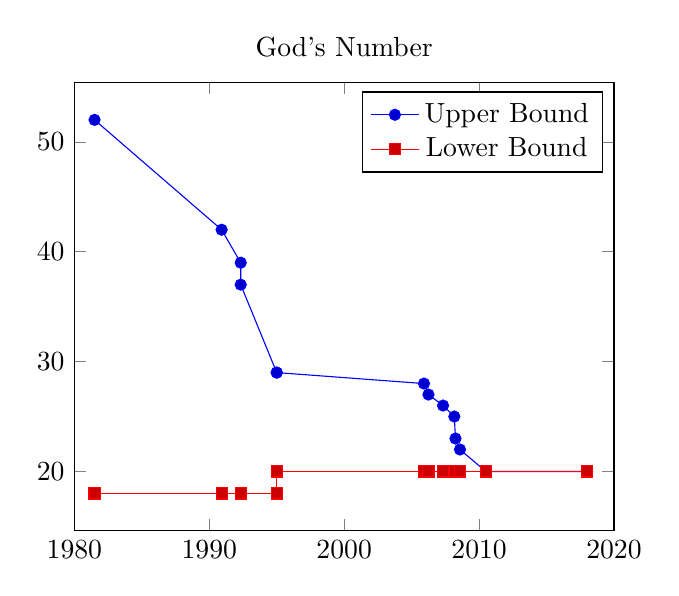
\begin{tikzpicture}
				\begin{axis}[title={God's Number}, date coordinates in=x,	enlarge x limits=false, xticklabel={\year},	date ZERO=1980-01-01, xmin=1980-01-01, xmax=2020-01-01,	xtick={1980-01-02,1990-01-01,2000-01-01,2010-01-01,2020-01-01}]
				\addplot coordinates {
					(1981-07-01, 52)
					(1990-12-01, 42)
					(1992-05-01, 39)
					(1992-05-01, 37)
					(1995-01-01, 29)
					(1995-01-01, 29)
					(2005-12-01, 28)
					(2006-04-01, 27)
					(2007-05-01, 26)
					(2008-03-01, 25)
					(2008-04-01, 23)
					(2008-08-01, 22)
					(2010-07-01, 20)
					(2018-01-01, 20)
				};
				\addplot coordinates {
					(1981-07-01, 18)
					(1990-12-01, 18)
					(1992-05-01, 18)
					(1992-05-01, 18)
					(1995-01-01, 18)
					(1995-01-01, 20)
					(2005-12-01, 20)
					(2006-04-01, 20)
					(2007-05-01, 20)
					(2008-03-01, 20)
					(2008-04-01, 20)
					(2008-08-01, 20)
					(2010-07-01, 20)
					(2018-01-01, 20)
				};
				\legend{Upper Bound, Lower Bound}
				\end{axis}
			\end{tikzpicture}
    		\caption{The upper bound was decreased to 20 over the course of twenty-nine years and across thirteen separate studies \cite{Rokicki2010}}
			\label{fig:godsnumbergraph}
		\end{center}
	\end{figure}

    
    \section{Python as a Scientific Scripting Language}
    Traditionally when performing large calculations and processes, compiled languages (C, C++, Fortran etc.) are the preferred choice over scripting languages such as Ruby, JavaScript, (pure) Python, etcetera. This is because compilation is done before run-time, allowing the program to run unhindered by on-the-fly translation/interpretation \cite{Cai2005}.
    
    For general purpose applications, scripting languages are preferable because they allow small changes to be made without re-compiling large classes before testing. In the thirteenth issue of \propernoun{Scientific Programming}, Cai, Langtangen and Moe \cite{Cai2005} explain how MATLAB is often a preferable choice for less intensive scientific computation due to its many features, such as: integrated simulation and visualisation tools; clear syntax; immediate feedback of commands; impressive documentation. They describe the use of MATLAB in computational science as paradoxical, as it is a scripting language which inherently is interpreted at run-time.
    
    One of MATLAB's biggest selling points, the IDE with integrated support for matrices, graphs and other mathematical features, can be replicated in a few Python IDEs or with the addition of Python packages. Python's main core can be expanded massively by using any of the tens of thousands of available packages, which can provide any of MATLAB's advantages alongside extra flexibility and capabilities. One of the most popular packages, \propernoun{Numerical Python} (NumPy), adds support for most scientific calculations. It expands Python's inbuilt data structures to use multi-dimensional homogeneous arrays of any Python data type. NumPy takes Python from a well-structured general-purpose language to a powerful mathematical language which can be applied to many different tasks \cite{Cai2005}, \cite{Oliphant2006}.
    
    As well as the multitude of available packages, Python has another major tool in its arsenal: it can be extended with a compiled language by design. This means that processor-intensive tasks like nested for loops can be migrated to a compiled language such as C++ or Fortran, increasing run speed up to a factor of ten. This extension process is now a trivial matter thanks to automated tools such as \propernoun{f2py}, which allows for automated calls to compiled Fortran code \cite{Oliphant2006}.
    
    \section{Conclusion}
    Lego Mindstorms is a strong candidate for the construction of the robot: its variable morphology allows adaptation to a range of tasks; the uniformity between pieces means that the main EV3 kit can be supplemented with other kits to extend its ability; and previous studies have shown that it is ideal for stimulating analysis and observations. Instead of using a single algorithm to solve the Cube, a range will be implemented in order to find the strongest method for finding a solve sequence. This will allow cross-comparison between, and analysis of, individual algorithms with the intention of finding the algorithm best suited to this project. Tree and group based algorithms alike will be implemented.
    
    MATLAB is incompatible with the Lego EV3, so will not be used for this project. Python's wide compatibility, clear high-level syntax, and extendibility to compiled code for more complex calculations, makes is the ideal language for this project. The main program will be written in Python, with any intensive processing written in C++ to improve the speed of the algorithms.
   
    \newpage
    \chapter{Requirements and Analysis}
    \epigraph{I have yet to see any problem, however complicated, which when you looked at in the right way, did not become still more complicated.}{Paul Anderson, New Scientist \cite{Anderson1969}}
    
    \section{Introduction} % TODO: maybe add more to this
    This chapter covers the specific requirements needed for the project to succeed: the particular tasks to complete the project; the hardware required to build the robot and run the solving program; and the software needed to write and run the program. As well as the requirements, an in-depth analysis of the project and its goals is made, discussing their feasibility, difficulty, and how necessary they are for the success of this project.
    
    \section{Specific Aims and Objectives}
    
    \begin{enumerate}
    	\item Build a robot which can manipulate a Cube accurately \par This is the first of the two primary objectives for this project, and is imperative to the project's success. As such it will be the first objective to be completed. This task, despite being of a medium difficulty, is fairly straightforward by nature: the robot simply needs to manipulate a Cube in any valid move.
    	\item Implement a system which successfully generates a solve sequence for any given position. \par The second primary objective ensures that any of the forty-three quintillion positions of Rubik's Cube can be solved correctly. The time taken to generate the solve sequence and the actual length of the solve sequence will both be used when measuring an algorithm's success.
    	\item When the robot is provided with a move sequence...
    	\begin{enumerate}
    		\item Convert any input sequence to be robot-compatible \par All of the pre-existing algorithms return a solution which a human being can follow to solve a real-world Cube. In the context of this project the manipulation is done by the robot, which cannot perform all of the standard moves, so any sequences provided must be translated to one which the robot can follow.
    		\item Correctly follow the sequence to achieve the intended output \par Once a robot-compatible move sequence has been generated, the robot must move the Cube in this exact sequence with no errors or move-failures. If a single move is performed incorrectly then the entire move sequence will produce an incorrect output.
    	\end{enumerate}
    	\item Ensure the runtime of the system is an acceptable length \par Previous solve sequence generator algorithms have had a run-time in the order of weeks: the desired run-time of the generation by this project will be in the order of minutes. This will require careful analysis of the trade off between generator efficiency and solve sequence length.
    	\item Implement a program to use a range of algorithms to generate a solve sequence \par In order to effectively compare the performance of several algorithms, there must be a method of running them under the same conditions and with the same overheads (e.g. transmission time to the robot). For this reason, there will be one main program with an option for the algorithm to use.
    	\item Compare the performance of different algorithms, especially the difference between human and robot compatible move sequences \par The performance of each algorithm will be tracked and compared fairly to show each one's merits and faults. This will allow the choice of one algorithm to be improved to create the most efficient method - or the potential combination of algorithms to form a stronger one.
    \end{enumerate}
    
    \section{Analysis}
    \subsection{Software}
    
    \subsubsection{PyCharm/CLion}
    An Integrated Development Environment (IDE) makes development, running programs, and testing and debugging much easier than using a simple text editor and command line. PyCharm and CLion by JetBrains \cite{JetBrains} will be used for developing in Python and C++ respectively. PyCharm and CLion provide strong code completion abilities, project-wide refactoring, and software development kit (SDK) modification amongst many other abilities. This will allow more time to be allocated to tasks of higher value rather than struggling with relatively minor issues.
    
	\subsubsection{Python 3.6 Runtime Environment}
    As discussed in the Literature Review, Python is the ideal language for this project. It requires a native runtime environment for programs to be run: this consists of the Python interpreter, libraries, and any packages used in the development process.
    
    \subsubsection{MinGW}
    C++ requires an environment to develop and compile in. MinGW (Minimalist GNU for Windows) is a popular choice when developing C++ applications. % TODO complete this
    
    \subsubsection{ev3dev}
    ev3dev \cite{Ev3dev.org} is a custom operating system (OS) for the EV3 which contains a low-level framework for the peripherals of an EV3. It allows users to write their own programs in a multitude of languages (including Python) to create complex functions and models. It is installed by flashing the ev3dev OS to a microSD card which is then inserted into the EV3, avoiding affecting the EV3's original firmware.
    
    A Python wrapper is available on GitHub \cite{Ev3dev} for the ev3dev OS, allowing the creation of Python programs with packaged support for the actuators and sensors of the EV3.
    
    \subsection{Software Requirements}
    This table shows the requirements of the software to be used in the creation of this project, and the capabilities of the computer that they will be running on. Any 
    
	\begin{table}[h]
		\def\arraystretch{1.25}
		\centering
		\caption{Software requirements for the main development computer and its capabilities}
		\label{tab:win_software}
		\begin{tabular}{M{0.18\textwidth}M{0.18\textwidth}M{0.18\textwidth}M{0.18\textwidth}M{0.18\textwidth}}
			\toprule
			\multirow{2}{*}{\tbo{Software}} & \multicolumn{4}{c}{\tbo{Requirements/Capabilities}} \\
			& \tbo{Minimum OS} & \tbo{Processor} & \tbo{Memory} & \tbo{Connectivity} \\
			\midrule
			PyCharm	&	Windows 2003 (or newer)	&		&	\normalsize{1GB} \scriptsize{minimum} \par \normalsize{2GB} \scriptsize{recommended} & \\
			CLion	&	Windows 7 64-bit (or newer)	&		&	\normalsize{2GB} \scriptsize{minimum}  & \\
			Lego EV3 Programming Software\cite{Lego2017}	&	Windows 2003 (or newer)	&	Dual Core 2GHz	&	2GB	&	1 USB Port \\
			Python 3.6	&	Windows Vista (or newer)	& &	& \\
			MinGW & \\
			\midrule
			\tit{Main Development Computer}	&	\tit{Windows 10 Pro 64-bit}	&	\tit{Quad Core i5 6500 3.6GHz}	&	\tit{32GB}	&	\tit{WiFi, Bluetooth, 12 $\times$ USB Port}\\
			\bottomrule
		\end{tabular}
	\end{table}
    
    \section{Feasibility Study}
    \subsection{Optimal Solutions}
	\subsection{Tree Based Methods}
    \subsection{Group Based Methods}
    
    \section{Evaluative Techniques}
    The progress of this project is estimated to follow the below Gantt Chart. For the duration of its lifespan, there will be a continual measurement of the actual progress against predicted.
    
	\begin{center}
		\begin{ganttchart}[title/.append style={fill=black!10}, hgrid, x unit=0.4mm, y unit title=7.5mm,, y unit chart=5mm, vgrid={*{6}{draw=none},dotted},	milestone/.append style={xscale=10}, time slot format=isodate]{2017-07-03}{2018-04-29}
			\gantttitlecalendar{year, month=shortname} \\
			\ganttgroup{Robot}{2017-07-15}{2017-09-18} \\
			\ganttbar{Design}{2017-07-20}{2017-08-20} \\
			\ganttbar{Build}{2017-08-08}{2017-09-04} \\
			\ganttbar{Testing}{2017-09-01}{2017-09-15} \\
			\ganttbar{Refinement}{2017-09-05}{2017-09-17} \\
			\ganttmilestone{Complete}{2017-09-18} \\
			\ganttgroup{Codebase}{2018-02-01}{2018-04-15} \\
			\ganttbar{Binary Search Method}{2018-02-05}{2018-02-25} \\
			\ganttbar{Primary Solve Method}{2018-02-24}{2018-03-05} \\
			\ganttmilestone{Cube Solved}{2018-03-05} \\
			\ganttbar{Primary Refinements}{2018-03-05}{2018-03-12} \\
			\ganttbar{Further Algorithms}{2018-03-10}{2018-03-20} \\
			\ganttbar{Performance Comparison}{2018-03-20}{2018-03-31} \\
			\ganttmilestone{Optimal Solve}{2018-04-05} \\
			\ganttbar{Implementation}{2018-03-16}{2018-04-04} \\
			\ganttbar{Testing}{2018-03-30}{2018-04-05} \\
			\ganttgroup{Final Write Up}{2017-09-20}{2018-04-29} \\
			\ganttbar{Introduction}{2017-09-23}{2017-10-02} \\
			\ganttbar{Research}{2017-09-28}{2017-12-12} \\
			\ganttbar{Literature Review}{2017-10-03}{2017-11-13} \\
			\ganttbar{Requirements and Analysis}{2017-10-28}{2017-11-20} \\
			\ganttbar{Results and Discussion}{2018-03-24}{2018-04-17} \\
			\ganttmilestone{Conclusions}{2018-04-20} \\
			\ganttmilestone{Deadline}{2018-05-02}
		\end{ganttchart}
	\end{center}
    
    \newpage
    
    \chapter[Design, Implementation and Testing]{Design, Implementation \\ and Testing}
    \epigraph{There are two ways of constructing a software design: One way is to make it so simple that there are obviously no deficiencies, and the other way is to make it so complicated that there are no obvious deficiencies. The first method is far more difficult.}{C.A.R. Hoare\cite{Hoare1981}}
    
	\section{Introduction}
	
	The nature of this project lends itself to a spiral design cycle, where both the robot and the solver can be designed, implemented, tested and then optimised to re-start the cycle. This non-linearity of the \tit{Design $\rightarrow$ Implementation $\rightarrow$ Testing} process means that the structure of this dissertation must follow the progress of the project, rather than having distinct sections for \enquote{Design} and \enquote{Implementation and Testing}. Consequentially this chapter's structure is split into two main parts - \enquote{Robot} and \enquote{Codebase} - each with introductory sections for fundamental components that are invariant through the different designs, and further sections to discuss each design.

	\begin{figure}[H]
		\begin{center}
			\includegraphics[width=0.3\textwidth]{Resources/Images/diagSpiralModel.png}
			\caption{The spiral model used for this project}
			\label{fig:diagSpiralModel}
		\end{center}
	\end{figure}

    \section{Robot Fundamentals and Prototyping}
    
    \subsection{Sensors and Actuators}
    
    The Lego EV3 comes with three DC motors (two large \legopiece{45502} and one medium \legopiece{45503}), a colour sensor and a touch sensor amongst other peripherals\footnote{The other peripherals are an infrared sensor and an infrared beacon, and are not used in this project.}. The quantity of the motors will be the largest restriction in designing the robot: it will only be able to rotate a Cube about two of the three axes; and the colour sensor will only have one degree of freedom so will rely on the rotation of the Cube to scan all of the facelets. The touch sensor can be used to allow limited user input to the robot at runtime, such as an emergency stop if the Cube becomes dislodged, or to confirm that the Cube is in place.
    
    \subsection{Prototyping with Lego}
    
    The first step in designing the robot was to prototype some simple designs for holding a Cube and successfully manipulating it. The first concept design was to grip each face of the Cube, and use a large motor to power the \enquote{grippers}. The second large motor could control which gripper was being powered at any time. This would allow a strong manipulation of the Cube and mean no delay between the movement of different faces. Figure \ref{fig:imgPrototype} shows the initial prototype that was built to fit this design. Once it was built, it became apparent that it was actually an impossible design (or at least, impossible with Lego) because if one of the grippers rotated by a quarter turn, it would block two of the other faces from turning. This can been seen below, where the upper gripper is blocking the left-hand one from turning. The solution to this would be to have the grippers retract when they are not in use, however this would be very difficult - if not impossible - to achieve with the available Lego pieces.
    
    \begin{figure}[H]
		\centering
		\begin{subfigure}[b]{0.30675\textwidth}
			\includegraphics[width=\textwidth]{Resources/Images/imgPrototype.jpg}
			\caption{The first prototype}
			\label{fig:imgPrototype}
		\end{subfigure}
		\hspace{10mm}
		\begin{subfigure}[b]{0.44325\textwidth}
			\includegraphics[width=\textwidth]{Resources/Images/imgCradleTest.jpg}
			\caption{The model used to test the motor's torque}
			\label{fig:imgCradleTest}
		\end{subfigure}
		\caption{A cross-section of the cradle and Cube}
		\label{fig:imgPrototypes}
	\end{figure}

	One of the other problems with the first prototype was that the Cube was unbalanced and would often fall out of the robot. This led to the design to have a \enquote{cradle} for the Cube to sit in. This is a good support mechanism for the Cube, and also handle the rotation about the Y axis. Once the cradle was built, it was a good milestone to check that the large motors had enough torque to rotate the face of a Cube against the friction between faces and slices. The motor was set to rotate indefinitely with the Cube in the cradle (as seen in Figure \ref{fig:imgCradleTest}) and the \slice{l-r} manually held in place. There was no visible reduction in the rotational velocity of the motor, so this first small test was passed.
	
	Although the cradle was a good solution to the problem outlined above, it also meant that only the \face{d} could be rotated, therefore requiring a mechanism to \enquote{flip} the Cube in place so different faces could sit in the cradle. The most obvious design for this was to apply a force at the upper corner to create a resultant force to pivot about the wall of the cradle. This is shown by the free body diagram in Figure \ref{fig:dwgCubeFreeBodyDiagram}: the force $F$ will be applied by a mechanism powered by the second large motor; this will be combined with the resistive force $R$ of the cradle wall; the resultant force (shown in red) will be about the pivot point (also in red) to rotate the Cube. Once the Cube is partially out of the cradle, it will slide back into place due to the height difference between the wall and the base of the cradle, and the low coefficient of friction between the plastic of the Cube and the Lego pieces.
    
	\begin{figure}[H]
    	\begin{center}
    		\includegraphics[width=0.35\textwidth]{Resources/Images/dwgCubeFreeBodyDiagram.png}
    		\caption{A free body diagram showing how the Cube will be rotated}
    		\label{fig:dwgCubeFreeBodyDiagram}
    	\end{center}
    \end{figure}
    
    \subsection{Fundamental Component Definitions} \label{sec:componentDefinitions}
    
    Following the construction and analysis of small Lego prototypes, it became apparent that there would be three fundamental components for the archetypal robot: a cradle would be needed to hold the Cube and rotate about the Y axis; an arm to rotate the Cube about the X axis and hold it in place for performing \move{d}s; and a moving arm for the colour sensor to scan the Cube. The essential requirements for these components are described below.
    
    \subsubsection{Cradle}
    
    The Cube will sit in a cradle which rotates about the Y axis to provide the movement needed for the moveset \moveset{Y.Y'y2D.D'd2}. This will have an inner dimension of 7 studs $\times$ 7 studs (56 \si{\milli\metre} $\times$ 56 \si{\milli\metre}) to closely match the dimensions of the Valk 3: 55.5 \si{\milli\metre} $\times$ 55.5 \si{\milli\metre} $\times$ 55.5 \si{\milli\metre}. The 0.5 \si{\milli\metre} tolerance means that the Cube doesn't have to be absolutely perfectly aligned when it is rotated (i.e. the program won't fail if the cube is a degree out of line). The cradle must rotate as accurately as possible to 90$\degree$ increments to ensure the success of the \move{x}s and avoid the Cube falling out of the cradle. 
    
    \subsubsection{X-Move Arm}
    To perform an \move{x}, some kind of arm will need to \enquote{flip} the Cube about its X axis. This should be a quick movement, with high reliability and good structural soundness. The arm must not interfere with the other components of the robot at any point. Furthermore the arm will also need to incorporate functionality to hold the \slice{l-r} and the \face{u} in place whilst the cradle rotates to perform a permutation of the \move{d}.
    
    \subsubsection{Colour Sensor}
    The colour sensor will be attached to the end of an extending arm which can be moved by a rack and worm gear to ensure the sensor can be accurately placed above the correct facelet. The worm gears will have to be driven by the medium sized motor, which produces less torque than the large motors but has a larger maximum rotational velocity - making it ideal for overcoming the inherent speed reduction of the worm gears. The colour sensor will be in a fixed position relative to the arm, and will be centred relative to the Cube.
    
    \section{Robot Design MkI}
    
	When designing the first version of the robot (hereinafter referred to as the \tbo{MkI}), there was a clear hierarchy of components and an inherent build order: the \move{x} arm relied on the cradle to rotate the cube; and the colour sensor relied on both the arm and the cradle to rotate the cube for the scanning process. The design process for the components comprised technical drawings, followed by a real-world build and the concurrent creation of a virtual 3D model using BrickLink's Stud.io software \cite{BrickLink2016}. Rendered images of the virtual model are displayed below alongside the technical drawings to show the finer details of the mechanism and as evidence of the consideration used in the design of the MkI.
    
	\subsection{Cradle}
	
	The cradle is a solid base of 7 studs $\times$ 7 studs $\times$ 2 studs (length $\times$ breadth $\times$ height) with a surrounding wall with a height and depth of 1 stud. This ensures that the weight of the cradle is uniformly distributed and the centre of gravity is low. These are important factors in the design of the cradle because a potential design is for it to be mounted on a singular vertical shaft, which is quite flexible under relatively low amounts of strain. The upper layer of the cradle's base has a smooth solid surface - as opposed to the sides of Lego Technic pieces which have lots of holes - to allow the Cube to slide properly when moved out of the cradle for an \move{x}; and the lower layer provides an interface to allow mounting on either a vertical shaft or otherwise.
	
	\begin{figure}[H]
		\begin{center}
			\includegraphics[width=0.4\textwidth]{Resources/Images/rdrCradle.png}
			\caption{A view of the cradle with some parts removed}
			\label{fig:rdrCradle}
		\end{center}
	\end{figure}
	
	
	The wall will have a semi-circular profile to allow the Cube to rotate smoothly out of the base of the cradle as demonstrated in Figures \ref{fig:dwgCradleCurvedEdgeNormal} and \ref{fig:dwgCradleCurvedEdgeTilted}. The curved edge will also allow the Cube to slide back into the cradle completely, rather than resting on the upper corner of the edge piece. The method for rotating the cradle is for it to be mounted directly (with no gear train or intermediary mechanism) onto the rotor of a large motor. This gives it stability from the secure mount, high rotational velocity because there is no gearing down, and it will be accurate due to the in-built tachometer which provides \enquote{precise control to within one degree of accuracy} \cite{Lego}. Figure \ref{fig:dwgCradleProfileV1} shows the cradle mounted on the rotor via a large gear, which allows a strong interface with the motor and gives the cradle sufficient clearance from the motor to make a full rotation without collision.
    
    \begin{figure}[H]
    	\centering
 	   	\begin{subfigure}[b]{0.2\textwidth}
    		\includegraphics[width=\textwidth]{Resources/Images/dwgCradleCurvedEdgeNormal.png}
    		\caption{Resting position}
    		\label{fig:dwgCradleCurvedEdgeNormal}
    	\end{subfigure}
    	\hspace{10mm}
    	\begin{subfigure}[b]{0.2\textwidth}
    		\includegraphics[width=\textwidth]{Resources/Images/dwgCradleCurvedEdgeTilted.png}
    		\caption{Starting an \move{x}}
    		\label{fig:dwgCradleCurvedEdgeTilted}
    	\end{subfigure}
	    \hspace{10mm}
	    \begin{subfigure}[b]{0.4\textwidth}
	    	\includegraphics[width=\textwidth]{Resources/Images/dwgCradleProfileV1.png}
	    	\caption{The cradle is mounted on a motor}
	    	\label{fig:dwgCradleProfileV1}
	    \end{subfigure}
    	\caption{Technical drawgins showing the the Cube, the cradle, and its mounting}
    	\label{fig:CradleDrawings}
    \end{figure}    
    
    Figure \ref{fig:rdrCradleMountedRotor}, below, is a rendered image of the 3D aforementioned model. It shows how the cradle and the motor will be supported by a framework which will link to the rest of the MkI. The main body of the motor is supported both vertically and horizontally to stop it from leaning under its own weight and also to prevent the motor rotating due to the inertia of the Cube.
    
    \begin{figure}[H]
    	\begin{center}
    		\includegraphics[width=0.5\textwidth]{Resources/Images/rdrCradleMountedRotor.png}
    		\caption{A render showing the original cradle mount design}
    		\label{fig:rdrCradleMountedRotor}
    	\end{center}
    \end{figure}
    
    \subsection{X-Move Arm}
    
    To rotate the Cube about the X axis, a rotating arm will apply the force $F$ shown in \ref{fig:dwgCubeFreeBodyDiagram} to cause the Cube to pivot about the opposite cradle wall. The Cube will then slide back into the cradle to complete the rotation. On one end of the arm there will be a wheel with a rubber tire to provide enough friction to tip the Cube over, and the other end will have a set of guards which can hold the top two slices of the Cube in place when performing a \move{D} or \move{d'}. The length of the guards will be staggered so that they don't collide with the cradle mid-rotation. Small right-angled pieces have been used to reinforced the corners of the arm, and liftarms will be used to hold the guards together to resist the outwards pushing force exerted on them by the rotating Cube. The design of the arm and its positioning relative to the cradle can be seen in Figure \ref{fig:dwgRotatingArm}.
    
    \begin{figure}[H]
    	\begin{center}
    		\includegraphics[width=0.4\textwidth]{Resources/Images/dwgRotatingArm.png}
    		\caption{The rotating arm used to flip the Cube}
    		\label{fig:dwgRotatingArm}
    	\end{center}
    \end{figure}

	Three primary positions of the arm can be seen below in Figure \ref{fig:rdrXMoveArmV1}. Figure \ref{fig:rdrXMoveArmV1_1} shows the \enquote{guarded} position of the arm, where the guards are positioned either side of the Cube to hold the \slice{l-r} and the \face{U} in place when performing a \move{D}, \move{D'} or \move{D2}. The two liftarms \legopiece{40490} that have been attached to the upper part of the guards to hold them together are visible just above the right-angled connectors \legopiece{55615} used to attach the guards to the arm. The guard assembly is attached to a central axle which is rotated by the large motor visible at the far side of the model. The entire assembly's weight is balanced sufficiently well to ensure that there is a smooth rotation about the axle and no unnecessary strain is placed on the motor.

	\begin{figure}[H]
		\centering
		\begin{subfigure}[b]{0.22193\textwidth}
			\includegraphics[width=\textwidth]{Resources/Images/rdrXMoveArmV1_1.png}
			\caption{Guarded position}
			\label{fig:rdrXMoveArmV1_1}
		\end{subfigure}
		\hspace{10mm}
		\begin{subfigure}[b]{0.22\textwidth}
			\includegraphics[width=\textwidth]{Resources/Images/rdrXMoveArmV1_2.png}
			\caption{Starting the \move{X}}
			\label{fig:rdrXMoveArmV1_2}
		\end{subfigure}
		\hspace{10mm}
		\begin{subfigure}[b]{0.30811\textwidth}
			\includegraphics[width=\textwidth]{Resources/Images/rdrXMoveArmV1_3.png}
			\caption{Unguarded position}
			\label{fig:rdrXMoveArmV1_3}
		\end{subfigure}
		\caption{Three different positions of the X-Move Arm}
		\label{fig:rdrXMoveArmV1}
	\end{figure}
	

	\subsection{Colour Sensor}
	
	\subsubsection{Lego Design}
	
	The colour sensor will be powered by the medium motor and a gear train which ends with a worm gear and rack \legopiece{3743}. The rack will be directly connected to a liftarm which has two long parallel shafts \legopiece{3708} mounted above it, both of which feed through a liftarm attached to the main frame of the MkI. These shafts are the only fixed mounting points for the whole colour sensor assembly - the worm gears and rack provide lateral movement but little to no structural support. The distance between the sensor and the top of the Cube will be approximately 8 \si{\milli\metre}. From previous tests and forum data, the optimal distance for the colour sensor appears to be between 10 \si{\milli\metre} and 16 \si{\milli\metre} \cite{UlfR2015}. Although the chosen distance is less than optimal, it ensures that the \enquote{beam} from the colour sensor remains inside the facelets. The accuracy of the readings will not be affected.
	
	\begin{figure}[H]
		\begin{center}
			\includegraphics[width=0.5\textwidth]{Resources/Images/dwgColorSensor.png}
			\caption{The colour sensor mounting arm is driven by a set of worm gears}
			\label{fig:dwgColorSensor}
		\end{center}
	\end{figure}
	
	The medium motor powers a 24-tooth gear \legopiece{60c01}, which then transmits power to an 8-tooth gear \legopiece{3647}, which is on the same axle as the worm gears. The rotational velocity of the worm gear is 63.75 \si{\radian\per\second} (608 RPM), which means that a large 40-tooth gear would have a rotational velocity of 1.59 \si{\radian\per\second} (15.2 RPM). Using this rotational velocity, the surface velocity of the large gear and therefore the lateral velocity of the rack can be calculated to be $\sim$0.0662 \si{\meter\per\second}. Given that the range of the colour sensor assembly's moveable distance is 80 \si{\milli\metre}, the time taken for the colour sensor to travel from its neutral position to above the centre facelet is 1.21 \si{\second}. Whilst this may seem like a relatively long time for the motor to move a light load, the assembly will only have to make the full journey between each face and at the start and end of the scanning process.
	
	\begin{figure}[H]
		\centering
		\begin{subfigure}[b]{0.43427\textwidth}
			\includegraphics[width=\textwidth]{Resources/Images/rdrColorSensorAssembly.png}
			\caption{A full view of the mechanics}
			\label{fig:rdrColorSensorAssembly}
		\end{subfigure}
		\hspace{10mm}
		\begin{subfigure}[b]{0.4\textwidth}
			\includegraphics[width=\textwidth]{Resources/Images/rdrColorSensorShaftDetail.png}
			\caption{The assembly's mounting structure}
			\label{fig:rdrColorSensorShaftDetail}
		\end{subfigure}
		\caption{The colour sensor assembly}
		\label{fig:rdrColorSensor}
	\end{figure}
	
	Where the motors used for the cradle and the \move{x} arm can both rotate indefinitely without a mechanical issue (colliding with other parts of the MkI, for instance), the one powering the colour sensor cannot rotate indefinitely due to the limited freedom of the colour sensor assembly. When the assembly reaches the end of its travel, it will be stopped by the liftarm that holds the shafts, causing it to stop the gear train and in turn provide a level of resistance to the motor that could either damage the motor or force the MkI to break apart. For this reason, the 24-tooth gear \legopiece{60c01} (which is the first in the gear train) is a special type of \enquote{clutch gear}, shown in Figure \ref{fig:imgClutchGear}. This means that it will only transmit a maximum torque value of between 2.5 \si{\newton\centi\metre} and 5.0 \si{\newton\centi\metre}. The theoretical output torque of the gear train is 2.21 \si{\newton\centi\metre}, so the clutch gear will function as a regular gear for the duration of colour sensor movement. When the assembly reaches its limit, the resistance to the gear train will cause the clutch gear to slip and the motor can continue turning without damaging itself or the MkI. This all ensures that if an error occurs which causes the motor to remain in a running state, no components will be damaged. Clearly an error of that magnitude should never occur if \lstinline|try...except| statements are used correctly, but this is a final fail-safe measure.
	
	\begin{figure}
		\centering
		\begin{minipage}{0.4\textwidth}
			\centering
			\includegraphics[width=0.8\textwidth]{Resources/Images/imgClutchGear.jpg}
			\caption{The clutch gear used to protect the motor}
			\label{fig:imgClutchGear}
		\end{minipage}%
		\hspace{10mm}
		\begin{minipage}{0.4\textwidth}
			\centering
			\includegraphics[width=0.8\textwidth]{Resources/Images/dwgCubeProfileCentreArcs.png}
			\caption{A Cube, with arcs drawn at the centre points of the cubies}
			\label{fig:dwgCubeProfileCentreArcs}
		\end{minipage}
	\end{figure}
	
	Figure \ref{fig:dwgCubeProfileCentreArcs} shows that the radial distance between the centre points of the middle and corner cubies is 15.33 \si{\milli\metre}. The colour sensor will have to travel this distance forty-two times during the scanning process, as well as the distance to the centre six times, making the total theoretical travelling time of the colour sensor approximately 21.26 \si{\second}.

	\subsubsection{Algorithm Design}

	In order to scan a full Cube, the sequence \movesequence{X.X.X.Y.X.X.X} will be followed, and the \face{u} scanned every time a new face is seen, as shown by algorithms \ref{alg:scanupface} and \ref{alg:scancube}:
	
	\begin{algorithm}[H]
		\caption{Scanning the Up-Face of a Cube}\label{alg:scanupface}
		\begin{algorithmic}[1]
			\Function{scan\uscore up\uscore face}{}
			\State facelet\uscore list $\gets [\;]$\Comment{Initialise as empty list}
			\For{$i \gets 0$ \tbo{to} $4$}\Comment{4 Corner-Edge pairs}
			\State \Call{move\uscore color\uscore sensor}{edge\uscore cubie}
			\State facelet\uscore list $\gets$ color\uscore value
			\State \Call{rotate\uscore cradle}{45}
			\State
			\State \Call{move\uscore color\uscore sensor}{corner\uscore cubie}
			\State facelet\uscore list $\gets$ color\uscore value
			\State \Call{rotate\uscore cradle}{45}
			\EndFor
			\State \Call{move\uscore color\uscore sensor}{centre\uscore cubie}
			\State facelet\uscore list $\gets$ color\uscore value
			\State \tbo{return} facelet\uscore list
			\EndFunction
		\end{algorithmic}
	\end{algorithm}
	
	Algorithm \ref{alg:scanupface} is called six times by the main scanning process, and is used to move the cradle and the colour sensor to the correct position to scan each facelet in turn. In the algorithm, an empty list is declared for the nine facelets to be appended to. \lstinline|move_color_sensor| takes a single parameter: the stopping point for the motor. The variables \lstinline|edge_cubie|, \lstinline|corner_cubie| and \lstinline|centre_cubie| are all integer constants which are used as these stopping points. The motor is rotated until the tachometer value is \tit{greater than or} equal to the variable - or less than if it is rotating backwards - so that if it is rotating faster than one \enquote{tacho-unit} at a time, it will not skip the stopping variable and continue indefinitely.
	
	Similarly to \lstinline|move_color_sensor|, \lstinline|rotate_cradle| takes a single parameter - but not a stopping point. Rather, it is the value which the current position of the motor is to be incremented by, in degrees. This value will then be multiplied as necessary to account for the gear ratios to create an output rotation matching the provided angle.
	
	\begin{algorithm}[H]
		\caption{Scanning an entire Cube}\label{alg:scancube}
		\begin{algorithmic}[1]
			\Function{scan\uscore cube}{}
			\State faces $\gets [\;[\;], [\;], [\;], [\;], [\;], [\;]\;]$\Comment{Initialise as 6 empty lists}
			\For{i $\gets$ 0 \tbo{to} \Call{length}{faces}}
			\State faces[i] $\gets$ \Call{scan\uscore up\uscore face}{}
			\If{i == 3} 
			\State \Call{rotate\uscore cradle}{90}\Comment{Allows \face{l} and \face{r} to be scanned after \move{x}}
			\EndIf
			\If{i $<$ 5} 
			\State \Call{x\uscore move\uscore cube}{}\Comment{\move{x} the Cube to get a new Color on the \face{u}}
			\EndIf
			\If{i == 4} 
			\State \Call{x\uscore move\uscore cube}{}\Comment{Extra \move{x} to get to \face{d}}
			\EndIf
			\EndFor
			\State \tbo{return} faces
			\EndFunction
		\end{algorithmic}
	\end{algorithm}

	\subsection{Full Model}
	
	\begin{figure}[H]
		\begin{center}
			\includegraphics[width=0.9\textwidth]{Resources/Images/rdrFullRobotV1.png}
			\caption{The full robot assembly}
			\label{fig:rdrFullRobotV1}
		\end{center}
	\end{figure}
	
	Figure \ref{fig:rdrFullRobotV1} demonstrates the full assembly of the MkI, including the main EV3 control brick. This model is the final result after any modifications made during the building process. These modifications to the model were only made to reflect the lack of some Lego pieces and the substituted pieces, and only affected the framework of the model - not any of the mechanisms mentioned above. As a result of the in-depth design process and any minor modifications, the MkI was optimised as much as possible with regards to functionality, structural integrity, and efficiency to work under restrictions from piece availability.
	
	The build of the MkI is quite compact, and the design is largely influenced by the pieces available: during the modelling process, small sections of the model were built with actual Lego to check functionality translated from the virtual model to the physical model as intended. Due to the limited quantity of Lego pieces, some less-than-optimal sections arose where two parts had to be connected but the necessary liftarm was not available. This situation is visible behind the cradle, where six small red pieces \legopiece{32062} are used to connect two right-angled liftarms. Another example of \enquote{design by necessity} is in the colour sensor's gear train: one medium and two small gears were used consecutively instead of two medium, or one large and one small. The functional impact of some of these sections is negligible thanks to workarounds and extra pieces, however the aesthetics have unfortunately suffered minor setbacks in places.
	
	A touch sensor \legopiece{95648} is mounted on the side of the frame that surrounds the cradle and the X-Move Arm. This adds the ability for user input when the program is running, without needing to access the operating system through the control brick. Simple tasks can be bound to the button at each stage of the program (e.g. pause the scanning process if a move fails or confirm initialisation). The EV3 control brick is mounted on the side of the MkI to allow easy access to the controls which allow navigation of the file system and turning the brick on and off. It is held in place by several long pins \legopiece{32054} which can be easily retracted to allow quick removal of the brick so the batteries can be changed.

	\subsection{Implementation and Testing}
	
	The MkI was built according to the design specifications laid out above, with little to no modification throughout. To thoroughly test the functions of the MkI (and any subsequent designs), a simple algorithm was designed to test and optimise the motorised functions of the MkI.
	
	\begin{algorithm}[H]
		\caption{Testing the MkI's Functionality}\label{alg:mkITest}
		\begin{algorithmic}[1]
			\Function{test\uscore mk\uscore I}{}
			\State test\uscore pass $\gets$ false
			\Repeat
			\State \tit{Optimise Cube}\Comment{Either modify parameters for motors or do real-world optimisations}
			\State \Call{scan\uscore cube}{}
			\State \Call{robot\uscore move\uscore sequence}{\movesequence{y.y'x.y'd'd2d'x}}
			\State test\uscore pass $\gets$ (actual\uscore cube == expected\uscore cube)
			\Until{test\uscore pass}
			\EndFunction
		\end{algorithmic}
	\end{algorithm}

	The first part of the test was to run the scanning process from start to end, as described by Algorithms \ref{alg:scanupface} and \ref{alg:scancube}, to test the movement of all three fundamental components. The \lstinline|repeat...until| loop allows optimisations to be made between each test: for the first few runs, the optimisations were quite simple, such as refining the constants used for setting the stopping points for the components; further optimisations involved making small modifications to the MkI design to reinforce the framework, or changes to the rotational velocity of the motors amongst other changes. The second part of the loop (where the move sequence \movesequence{y.y'x.y'd'd2d'x} is run) allows the functionality of the MkI during the solving process to be tested. This covers the accuracy of the cradle for \move{d}s and \move{y}s, the accuracy and the effectiveness of the \move{x} arm's guards, and the success of the \move{x}s. Minor modifications that were easily solved are subsequently ignored for the sake of conciseness and efficiency.
	
	\subsubsection{Major Issues}
	
	The first major issue with the functionality of the MkI was actually software-based - however it is discussed here because it produced a hardware issue which affected the MkI's design. The details of the code used are discussed in section \ref{sec:ev3components}. In Algorithm \ref{alg:mkITest}, the stopping condition for the main loop is a comparison between the virtual Cube and the real-world Cube. This comparison was a manual one, where the position of the Cube was checked against an on-screen printout. The colour sensor has different modes to read colours: \lstinline|COL_COLOR|, which returns an integer between zero and seven (inc.) to represent a specific colour; \lstinline|RGB_RAW|, which returns the RGB values read by the sensor; and other modes which read light intensity rather than the colour. For this application, the \lstinline|COL_COLOR| is the most suitable mode because it will not require the RGB values to be parsed into one of the six colours.
	
	The only problem was, the on-screen printout was always a mix of blue, red and white rather than the expected mix of the usual six colours. The first solution to this problem was to change the magnitude of the space between the colour sensor and the top of the Cube: testing a number of distances between 5 \si{\milli\metre} and 25 \si{\milli\metre} produced the same colours, with slight variances in darkness and little else. To properly debug this problem, the mode was set to \lstinline|RGB_RAW| and the RGB values returned by the colour sensor were compared with values read by the camera on a OnePlus 3\footnote{A simple RGB colour picking app was used \cite{RangoApps2015}}.
	
   	\begin{table}[h!]
		\def\arraystretch{1.25}
		\centering
		\caption{A comparison of the colour values returned by a OnePlus 3 and the Lego Colour Sensor}
		\label{tab:coloursensor1}
		\begin{tabular}{M{0.1\textwidth}M{0.075\textwidth}M{0.075\textwidth}M{0.075\textwidth}M{0.07\textwidth}M{0.075\textwidth}M{0.075\textwidth}M{0.075\textwidth}M{0.07\textwidth}}
			\toprule
			\multirow{2}{*}{\tbo{Face}} & \multicolumn{4}{c}{\tbo{OnePlus 3}} 			& \multicolumn{4}{c}{\tbo{Lego Colour Sensor}}  \\
										& \tbo{Red}&\tbo{Green}&\tbo{Blue}&\tbo{RGB}	& \tbo{Red}&\tbo{Green}&\tbo{Blue}&\tbo{RGB} 	\\
			\midrule
			White	&229&224&221&\cellcolor[rgb]{0.90,0.88,0.87}	&79&106&53&\cellcolor[rgb]{0.31,0.42,0.21}\textcolor{white}{White}	\\	
			Yellow	&181&195&0  &\cellcolor[rgb]{0.71,0.76,0.00}	&73&97 &76&\cellcolor[rgb]{0.29,0.38,0.30}\textcolor{white}{White}	\\
			Red		&223&25 &35 &\cellcolor[rgb]{0.87,0.10,0.14}	&52&24 &9 &\cellcolor[rgb]{0.20,0.09,0.04}\textcolor{white}{Red}	\\
			Orange	&251&127&21 &\cellcolor[rgb]{0.98,0.50,0.08}	&68&93 &75&\cellcolor[rgb]{0.27,0.36,0.29}\textcolor{white}{White}	\\
			Green	&34 &186&8  &\cellcolor[rgb]{0.13,0.73,0.03}	&25&71 &48&\cellcolor[rgb]{0.10,0.28,0.19}\textcolor{white}{Blue}	\\
			Blue	&0  &130&255&\cellcolor[rgb]{0.00,0.51,1.00}	&10&31 &31&\cellcolor[rgb]{0.04,0.12,0.12}\textcolor{white}{Blue}	\\
			\bottomrule
		\end{tabular}
	\end{table}

	Table \ref{tab:coloursensor1} compares the values read by both sensors, along with the RGB values. The \lstinline|COL_COLOR| values have been overlaid on the colours returned by the Lego sensor to show how they are interpreted by ev3dev. After many more tests, readings of different surfaces, and hours of research, it became apparent that the issue was that the colour sensor wasn't capable of detecting fluorescent colours. Unfortunately, the Valk 3 only comes in fluorescent colours, a standard (darker) Rubik's branded Cube wouldn't fit in the cradle and has a lower build quality, and other speedcubes weren't a viable option mainly due to their cost.
	
	The solution to this problem was to print readable colours on standard white sticky labels and apply them over the stickers which were being incorrectly read (only the yellow, green and orange sides) on the Valk 3. The end result is visible in Figure \ref{fig:imgCubeStickersComparison}, next to a non-stickered Valk 3 (a variation with no black borders, but still the same type of Cube). The orange side has been replaced with brown stickers because the colour sensor reads the five other colours, and then brown - not orange. For the duration of this project however, the colour will be referred to as orange for consistency.

	\begin{figure}[H]
		\begin{center}
			\includegraphics[width=0.5\textwidth]{Resources/Images/imgCubeStickersComparison.jpg}
			\caption{Side-by-side comparison of the Valk 3 with and without stickers}
			\label{fig:imgCubeStickersComparison}
		\end{center}
	\end{figure}

	Table \ref{tab:coloursensor2} shows that the new stickers greatly improved the accuracy of the colour sensor's readings. Although the colours in the final column of the table are all very dark and almost indistinguishable, the colour sensor apparently has no difficulty in telling the colours apart: approximately 500 facelets were scanned, and none were scanned incorrectly. As such, the sensor's accuracy with the new stickers is sufficient for this project.
	
   	\begin{table}[h!]
		\def\arraystretch{1.25}
		\centering
		\caption{A comparison of the colour values returned before and after the application of coloured stickers}
		\label{tab:coloursensor2}
		\begin{tabular}{M{0.1\textwidth}M{0.075\textwidth}M{0.075\textwidth}M{0.075\textwidth}M{0.07\textwidth}M{0.075\textwidth}M{0.075\textwidth}M{0.075\textwidth}M{0.07\textwidth}}
			\toprule
			\multirow{2}{*}{\tbo{Face}} & \multicolumn{4}{c}{\tbo{Original Stickers}} 			& \multicolumn{4}{c}{\tbo{Modified Stickers}}  \\
			& \tbo{Red}&\tbo{Green}&\tbo{Blue}&\tbo{RGB}	& \tbo{Red}&\tbo{Green}&\tbo{Blue}&\tbo{RGB} 	\\
			\midrule
			White	&79&106&53&\cellcolor[rgb]{0.31,0.42,0.21}\textcolor{white}{White}	&75&101&51&\cellcolor[rgb]{0.29,0.40,0.20}\textcolor{white}{White}	\\
			Yellow	&73&97 &76&\cellcolor[rgb]{0.29,0.38,0.30}\textcolor{white}{White}	&58&46 &8 &\cellcolor[rgb]{0.23,0.18,0.03}\textcolor{white}{Yellow}	\\
			Red		&52&24 &9 &\cellcolor[rgb]{0.20,0.09,0.04}\textcolor{white}{Red}	&41&18 &5 &\cellcolor[rgb]{0.16,0.07,0.02}\textcolor{white}{Red}	\\
			Orange	&68&93 &75&\cellcolor[rgb]{0.27,0.36,0.29}\textcolor{white}{White}	&24&14 &5 &\cellcolor[rgb]{0.09,0.05,0.02}\textcolor{white}{Orange}	\\
			Green	&25&71 &48&\cellcolor[rgb]{0.10,0.28,0.19}\textcolor{white}{Blue}	&11&33 &7 &\cellcolor[rgb]{0.04,0.13,0.03}\textcolor{white}{Green}	\\
			Blue	&10&31 &31&\cellcolor[rgb]{0.04,0.12,0.12}\textcolor{white}{Blue}	&9 &24 &17&\cellcolor[rgb]{0.04,0.09,0.06}\textcolor{white}{Blue}	\\
			\bottomrule
		\end{tabular}
	\end{table}

	Following more tests, it becamse clear that the addition of the stickers was a double-edged sword: the coefficient of friction between the Cube and the curved edge of the cradle wall was now too high for the Cube to slide back into the cradle following an \move{x}. If the \face{d} had any of the new stickers on, it would stay rested on the wall of the cradle and corrupt the entire process. Rather than spend time redesigning the cradle to be angled to make the Cube slide back in, or changing the arm design to pull the Cube back in, the easiest solution was simply to tilt the entire robot:
	
	\begin{figure}[H]
		\begin{center}
			\includegraphics[width=0.5\textwidth]{Resources/Images/imgCubeSolverV1.png}
			\caption{The MkI had a distinctive tilt to ensure the success of \move{x}s}
			\label{fig:imgCubeSolverV1}
		\end{center} 
	\end{figure}

	The second major issue with the MkI was in part caused by the newly added tilt, and also by the design of the \move{x} arm: when the wheel on the end of the arm pushed the Cube to start an \move{x}, the Cube would fall out of either side of the cradle instead of pivoting about the opposite wall. The main cause of this was that the wheel was exerting a force in the exact centre of the Cube's face, and the opposite wall was now higher (because of the added tilt) which meant that the resistive force was greater. There was no obvious solution to this problem, other than making the wheel larger to spread the force across the face of the Cube. However, a larger wheel meant that the arm became unbalanced and the strength of the arm was compromised. This led to the liftarm that held the wheel falling off the MkI mid-process more than once, as shown in Figure \ref{fig:mkIArmCollapse} (three frames extracted from a video of the scanning process).

	\begin{figure}[H]
		\centering
		\begin{subfigure}[b]{0.25\textwidth}
			\includegraphics[width=\textwidth]{Resources/Images/mkIArmCollapse1.png}
		\end{subfigure}
		\hspace{5mm}
		\begin{subfigure}[b]{0.25\textwidth}
			\includegraphics[width=\textwidth]{Resources/Images/mkIArmCollapse2.png}
		\end{subfigure}
		\hspace{5mm}
		\begin{subfigure}[b]{0.25\textwidth}
			\includegraphics[width=\textwidth]{Resources/Images/mkIArmCollapse3.png}
		\end{subfigure}
		\caption{The MkI \move{x} arm broke under greater resistance}
		\label{fig:mkIArmCollapse}
	\end{figure}
	
	The final issue with the MkI, which prompted a complete rebuild, was an inherent issue with the large motor that rotated the cradle. As with all DC motors, there is a slight amount of \enquote{play} in the rotor: it has a few degrees of freedom either side of its current position. This is usually not a problem, but because the cradle requires very high accuracy it can cause a complete failure for any part of the process. The play in the motor reduced the accuracy of the cradle, as it effectively introduced a zero error for each rotation. If the cradle only rotated in one direction then the zero error would only have to be offset at the very start of the program because the cradle would \enquote{sit} at one end of the region of play. However, this would have reduced the size of the available moveset by 50\% and thus have had a worst case runtime increase of 100\% (Sequentially, $|\movesequence{D'X}| = 2$ would have changed to $|\movesequence{D.D.D.X}| = 4$). A problem of this magnitude required a full analysis and re-design of the robot.

	\newpage
    \section{Robot Design MkII}
	\subsection{Improvements on MkI}
	Aside from the few major issues outlined above, the time spent testing and using the MkI led to the discovery of many more smaller issues that would be addressed during the design of the second iteration of the robot's design: the MkII. These minor issues are discussed below, as proof of the careful consideration used and to validate the choices made in designing the MkII.
	
	\subsubsection{Motor Initialisation}
	
	During the testing and general usage of the MkI, there were many occurrences of a fatal runtime error which would leave the motors out of their starting position. The usual cause of this was a \lstinline|StallError| from one of the motors or the voltage supply from the batteries becoming too low. The incorrect positioning required the motors to be initialised when restarting the program. To assist in this procedure, large black gears were added to the motors which allows them to be returned to their respective initial positions. A method was also added to the program disable the active braking on the motors so they weren't damaged when being rotated.
	
	\begin{figure}[H]
		\centering
		\begin{subfigure}[b]{0.25\textwidth}
			\includegraphics[width=\textwidth]{Resources/Images/rdrInitialiser1.png}
			\caption{Colour Sensor initialiser}
			\label{fig:rdrInitialiser1}
		\end{subfigure}
		\hspace{10mm}
		\begin{subfigure}[b]{0.25\textwidth}
			\includegraphics[width=\textwidth]{Resources/Images/rdrInitialiser2.png}
			\caption{Cradle initialiser}
			\label{fig:rdrInitialiser2}
		\end{subfigure}
		\hspace{10mm}
		\begin{subfigure}[b]{0.25\textwidth}
			\includegraphics[width=\textwidth]{Resources/Images/rdrInitialiser3.png}
			\caption{\move{x} Arm initialiser}
			\label{fig:rdrInitialiser3}
		\end{subfigure}
		\caption{The initialising gears used for each motor}
		\label{fig:rdrInitialiser}
	\end{figure}
	
	\subsubsection{Fragility and Adaptability}
	
	One of the MkI's greatest flaws was the fragility of the frame that held the \move{x} arm in place. It was also very difficult to make any adjustments to the MkI because of the complexity of the design. With this in mind the MkII was constructed of two main modules, each of which could be structurally tested independently. These modules were then connected with seven red pins \legopiece{32054} that are easily accessible: if any modifications need to be made to the MkII, the pins can be removed and the modules separated for quick and efficient modification.
	
	\begin{figure}[H]
		\centering
		\begin{subfigure}[b]{0.25\textwidth}
			\includegraphics[width=\textwidth]{Resources/Images/rdrModulePins1.png}
			\label{fig:rdrModulePins1}
		\end{subfigure}
		\hspace{10mm}
		\begin{subfigure}[b]{0.25\textwidth}
			\includegraphics[width=\textwidth]{Resources/Images/rdrModulePins2.png}
			\label{fig:rdrModulePins2}
		\end{subfigure}
		\hspace{10mm}
		\begin{subfigure}[b]{0.25\textwidth}
			\includegraphics[width=\textwidth]{Resources/Images/rdrModulePins3.png}
			\label{fig:rdrModulePins3}
		\end{subfigure}
		\caption{The pins used for connecting the modules}
		\label{fig:rdrModulePins}
	\end{figure}
	
	\subsubsection{Battery Usage}
	
	The final of the issues discovered by repeated testing of the MkI was how power-hungry the EV3 control brick really is. After only one to one-and-a-half hours of testing, it would run six AA 2500 \si{\milli\ampere\hour} batteries completely flat. Lego do sell a rechargeable battery for the EV3, however is is only 2050 \si{\milli\ampere\hour} by itself and its costs \pounds81.99 \cite{Lego2018}. A cheaper (and higher capacity) option was to purchase twelve rechargeable 2500 \si{\milli\ampere\hour} batteries and a charger for approximately \pounds25. Whilst the EV3 was voraciously consuming the power from six of the batteries, the other six could either be charging or waiting ready. This led to the design and creation of a battery holder attached to the MkII. It holds six AA batteries and has two pins which can be removed to release the batteries, as shown in Figure \ref{fig:imgBatteryHolderOpen}.
	
	\begin{figure}[H]
		\centering
		\begin{subfigure}[b]{0.27665\textwidth}
			\includegraphics[width=\textwidth]{Resources/Images/rdrBatteryHolder.png}
			\caption{The design of the battery holder, rendered}
			\label{fig:rdrBatteryHolder}
		\end{subfigure}
		\hspace{10mm}
		\begin{subfigure}[b]{0.21082\textwidth}
			\includegraphics[width=\textwidth]{Resources/Images/imgBatteryHolder.jpg}
			\caption{Six AA batteries ready for use}
			\label{fig:imgBatteryHolder}
		\end{subfigure}
		\hspace{10mm}
		\begin{subfigure}[b]{0.26253\textwidth}
			\includegraphics[width=\textwidth]{Resources/Images/imgBatteryHolderOpen.jpg}
			\caption{The battery holder is opened by removing the pins}
			\label{fig:imgBatteryHolderOpen}
		\end{subfigure}
		\caption{The battery holder, as a rendered model and in real life}
		\label{fig:batteryHolder}
	\end{figure}
	
	\subsection{Cradle}

	The MkI implementation of the cradle largely failed because of the play in the large motor upon which it was mounted. The accuracy of the motor was reduced and the rotations made unreliable. A worm gear \legopiece{4716} has solved both of these problems: it has been combined with a large gear \legopiece{3649} to create a gear ratio of 1:40, increasing the accuracy of the motor by a factor of forty (see Figure \ref{fig:dwgCradleWormGear}). This also slowed the maximum rotational velocity of the cradle to 0.209 \si{\radian\per\second} (2 RPM) at 7.5\si{\volt}, so a 90$\degree$ turn will take 7.5 seconds\footnote{This figure is the result of a measurement of the maximum rotational velocity of a large motor, and will fluctuate depending on the voltage supplied by the batteries in the EV3 brick}. A compromise between maximum rotational velocity and accuracy has been found by adding more gears to reduce the ratio. The problem presented by the play in the motor has been successfully minimised due to the unidirectional nature of the gear train.
	
	\begin{figure}[H]
		\centering
		\begin{subfigure}[b]{0.37999\textwidth}
			\includegraphics[width=\textwidth]{Resources/Images/dwgCradleWormGear.png}
			\caption{The rotation of the worm gear drives the cradle’s rotation}
			\label{fig:dwgCradleWormGear}
		\end{subfigure}
		\hspace{10mm}
		\begin{subfigure}[b]{0.42014\textwidth}
			\includegraphics[width=\textwidth]{Resources/Images/rdrCradleWormGear.png}
			\caption{The gear train which provides power to the cradle}
			\label{fig:rdrCradleWormGear}
		\end{subfigure}
		\caption{The battery holder, as a rendered model and in real life}
		\label{fig:cradleWormGear}
	\end{figure}
	
	Figure \ref{fig:rdrCradleWormGear} shows how the cradle is driven by a large motor. A large 36-tooth gear \legopiece{32498} is directly attached to the rotor with two small pins to reduce the need for an extended shaft which will flex when placed under strain (i.e. at the start of a rotation). This gear drives a 12-tooth gear \legopiece{32270} to triple the rotational velocity at that point of the gear train. This connection is immediately repeated and used to create a 90$\degree$ turn onto the shaft with the worm gear. At this point the speed ratio between the worm gear and the motor is 9:1, which is then decreased forty times by the large 40-tooth gear to create a final ratio of 1:4.444. This means the maximum rotational velocity of the cradle will be 1.843 \si{\radian\per\second} (17.6 RPM) at 7.5\si{\volt} and the original torque is increased from 17.3 \si{\newton\centi\metre} to 76.8 \si{\newton\centi\metre}, which will allow a face of the Cube to be rotated with ease. The vertical black shaft seen at the top of the image provides a mounting point for the cradle.
	
	\subsection{X-Move Arm}
    
    The largest change between the two design iterations was the complete update of the \move{x} arm - in functionality, aesthetics, and reliability. Where the MkI \move{x} arm relied on pushing the Cube, the MkII \tit{pulls} the Cube towards it. This creates a much more controlled movement, as the Cube is bound on all four sides at all times. As shown in Figure \ref{fig:rdrXMoveBlock}, the Cube cannot fall out of the cradle during the \enquote{pull} part of the rotation due to the small right-angled piece behind the cradle. The pulling motion causes the Cube's rotation, then the Cube is immediately pushed back into the cradle to complete the move.
   	
	\begin{figure}[H]
   		\begin{center}
   			\includegraphics[width=0.4\textwidth]{Resources/Images/rdrXMoveBlock.png}
   			\caption{A side elevation to show the pieces which block the Cube from falling}
   			\label{fig:rdrXMoveBlock}
   		\end{center} 
   	\end{figure}
   
    The arm is controlled by a single large motor, and is suspended from a tall frame by a liftarm which is free to pivot at both ends. This means that the arm can move \tit{along} the Z-axis as well as about the X-axis - albeit with limited freedom. Figure \ref{fig:rdrXMoveRenders} show the incremental steps for an \move{x}: 
    
    \begin{enumerate}[label=\alph*]
    	\item Starting position, the front of the arm is just touching the \face{f}
    	\item Maximum pull position, the Cube has rotated and is resting on the block piece from Figure \ref{fig:rdrXMoveBlock}
    	\item The Cube is pushed back into the cradle
    	\item Push is completed
    	\item The arm moves out of the way to end the \move{x}
    \end{enumerate}
    
   	\begin{figure}[H]
    	\centering
    	\begin{subfigure}[b]{0.25\textwidth}
    		\includegraphics[width=\textwidth]{Resources/Images/rdrXMoveArmLowered.png}
    		\caption{}
    		\label{fig:rdrXMoveArmLowered}
    	\end{subfigure}
    	\hspace{10mm}
    	\begin{subfigure}[b]{0.25\textwidth}
    		\includegraphics[width=\textwidth]{Resources/Images/rdrXMoveArmPulling.png}
    		\caption{}
    		\label{fig:rdrXMoveArmPulling}
    	\end{subfigure}
    	\hspace{10mm}
    	\begin{subfigure}[b]{0.25\textwidth}
    		\includegraphics[width=\textwidth]{Resources/Images/rdrXMoveArmLowered.png}
    		\caption{}
    		\label{fig:rdrXMoveArmLowered2}
    	\end{subfigure}
    	\begin{subfigure}[b]{0.25\textwidth}
    		\includegraphics[width=\textwidth]{Resources/Images/rdrXMoveArmPostPush.png}
    		\caption{}
    		\label{fig:rdrXMoveArmPostPush}
    	\end{subfigure}
    	\hspace{10mm}
    	\begin{subfigure}[b]{0.25\textwidth}
    		\includegraphics[width=\textwidth]{Resources/Images/rdrXMoveArmRaised.png}
    		\caption{}
    		\label{fig:rdrXMoveArmRaised}
    	\end{subfigure}
    	\caption{The steps of an \move{x}, in order}
    	\label{fig:rdrXMoveRenders}
    \end{figure}
    
    
    \subsection{Colour Sensor}
    
    The colour sensor was undoubtedly the most successful component of the MkI, and very little has been changed between design iterations. The clutch gear \legopiece{60c01} used in preventing any damage to the motor of the MkI framework actually became a hindrance: if the assembly encountered any resistance when moving (e.g. when the rack moves onto the second worm gear), then the clutch would slip and then the whole assembly would be out of line. This rarely caused incorrect scanning results, however it is easier to restrict damage by following good coding practices - which were developed with the use of the MkI - than with the clutch gear. The only other functional change to the colour sensor was the shortening of the axle which it rested on: the worm gear closest to the cradle was superfluous so was removed to avoid over-complicating the mechanism.
    
    \subsection{Full Model}
    
   	\begin{figure}[H]
    	\begin{center}
    		\includegraphics[width=0.9\textwidth]{Resources/Images/rdrMkIIFull.png}
    		\caption{The full MkII robot assembly}
    		\label{fig:rdrMkIIFull}
    	\end{center} 
    \end{figure}
    
    Figure \ref{fig:rdrMkIIFull} is the full assembly of the MkII. As with the full render of the MkI, the model has been updated to reflect any modifications made during the building process. The construction of the MkII is of much higher quality, with fewer shortcuts and workarounds used to make up for missing pieces. It is also considerably larger than the MkI due to the increased size of the \move{x} arm. The extended framework initially caused some flexing across the body of the MkII simply due to it's size and the forces exerted by the movement of the \move{x} arm. A very simple solution to this was to mount the entire MkII on \enquote{feet} made from wheels on their sides. The flexibility of the tyres allows the feet to act as dampers for the \move{x} arm, and the high friction between the tyres and the surface they sit on means that the MkII will not move around. The framework which the EV3 control brick is mounted on is actually mostly the same design as the MkI: this was one part there truly were no issues with. Reusing the framework meant less time had to be spent on the more mundane parts of the build, and more time could be spent getting the core components right. Once again, the touch sensor has been mounted on the front of the robot for easy access at runtime.
    
    \begin{figure}[H]
    	\centering
    	\begin{subfigure}[b]{0.275\textwidth}
    		\includegraphics[width=\textwidth]{Resources/Images/rdrMkIIElevation1.png}
    		\caption{}
    		\label{fig:rdrMkIIElevation1}
    	\end{subfigure}
    	\hspace{10mm}
    	\begin{subfigure}[b]{0.275\textwidth}
    		\includegraphics[width=\textwidth]{Resources/Images/rdrMkIIElevation2.png}
    		\caption{}
    		\label{fig:rdrMkIIElevation2}
    	\end{subfigure}
    	\hspace{10mm}
    	\begin{subfigure}[b]{0.275\textwidth}
    		\includegraphics[width=\textwidth]{Resources/Images/rdrMkIIElevation3.png}
    		\caption{}
    		\label{fig:rdrMkIIElevation3}
    	\end{subfigure}
    	\begin{subfigure}[b]{0.275\textwidth}
    		\includegraphics[width=\textwidth]{Resources/Images/rdrMkIIElevation4.png}
    		\caption{}
    		\label{fig:rdrMkIIElevation4}
    	\end{subfigure}
    	\hspace{10mm}
    	\begin{subfigure}[b]{0.275\textwidth}
    		\includegraphics[width=\textwidth]{Resources/Images/rdrMkIIElevation5.png}
    		\caption{}
    		\label{fig:rdrMkIIElevation5}
    	\end{subfigure}
		\hspace{10mm}
		\begin{subfigure}[b]{0.275\textwidth}
			\includegraphics[width=\textwidth]{Resources/Images/rdrMkIIElevation6.png}
			\caption{}
			\label{fig:rdrMkIIElevation6}
		\end{subfigure}
    	\caption{Elevation and plan views of the MkII}
    	\label{fig:rdrMkIIElevations}
    \end{figure}

    \subsection{Implementation and Testing}
    
	The implementation/building process of the MkII was fairly straightforward following the MkI's implementation. The more common errors and weaknesses in the design were easier to spot, and the knowledge gained from the previous design iteration greatly aided in making the MkII an all-round strong design. The use of the spiral model in designing the robot has generated a clear process from the design stage through to the testing stage, producing a robot with very few, if any, hardware-based bugs or issues.
	
	The definitions described in section \ref{sec:componentDefinitions} have been briefly quantified below for quick referencing:

	\subsubsection{Cradle}

	\begin{enumerate}
		\item The cradle should rotate about the Y axis to perform the moveset \moveset{Y.Y'y2D.D'd2} \label{lst:cr1}
		\item The cradle must rotate as accurately as possible to 90$\degree$ increments \label{lst:cr2}
		\item The Cube must not fall out of the cradle \label{lst:cr3}
	\end{enumerate}
	
	\subsubsection{X-Move Arm}
	
	\begin{enumerate}
		\item The \move{x} should be a quick movement \label{lst:x1}
		\item The \move{x} needs to be highly reliable and structurally sound \label{lst:x2}
		\item The arm must no interfere with other components \label{lst:x3}
		\item It must hold the \slice{l-r} and the \face{u} in place to perform a permutation of the \move{d} \label{lst:x4}
	\end{enumerate}
	
	\subsubsection{Colour Sensor}
	
	\begin{enumerate}
		\item The sensor must be able to be accurately positioned above the correct facelet \label{lst:cs1}
	\end{enumerate}

	Each of these definitions have been followed in the design of the robot, through thorough consideration of hardware capabilities and giving leaving plenty of room for improvement with both hardware and software. The MkI did not achieve items Cradle \ref{lst:cr2} and \ref{lst:cr3}, and \move{x} Arm \ref{lst:x2} so these were the largest changes as the spiral model progressed. The MkII, however, has successfully fulfilled all of the definitions with a very small margin of error. It has therefore been marked as a success, and will not be developed further.
    
    \newpage
    \section{Codebase}
    \subsection{EV3 Components} \label{sec:ev3components}
    \subsection{Object Classes}
    \subsubsection{Cube}
    \subsubsection{Position}
    \subsection{Solve Methods}
    \subsection{Method 1: Tree Solving}
	\subsection{Method 2: Group Solving}
    \subsection{Database}
    \subsection{Move Sequence Translation}
    
    The algorithms considered and discussed in the Literature Review (as well as others used in determining God's Number) are designed to work with a standard moveset \moveset{L.R.U.D.F.B} (as well as half turns and counter-clockwise turns). The design of the robot means that it is restricted to the moveset \moveset{X.Y.y'y2D.d'd2} - and will therefore require any incompatible sequences to be translated to the robot's moveset.
    
    When the entire Cube is rotated, the \tbo{colour} of the faces will change but the faces' \tbo{orientations} will not (analogous to when one turns on the spot: left and right have changed, but east and west have not). This means that the frame of reference for the moves will have to remain invariant throughout a sequence by compensating for any full Cube rotations.
    
    This is best explained with an example: the first step in performing the sequence \movesequence{u.f} would be to do perform \movesequence{x2d} in order to complete the \move{u}; but now that the original \face{f} has moved (due to the \movesequence{x2}) - it must be located, the Cube must be rotated to get the original \face{f} into the cradle, and then the sequence can be completed. The simplest method of overcoming this complication is to convert the original move sequence to an equivalent sequence of colour-based moves: \movesequence{u.f} $\equiv$ \movesequence{W.G}.
    
    Once the original sequence has been converted to a colour-based sequence, a deep copy of the original Cube is made and the coloured sequence is iteratively translated and applied to this Cube. On each element of the sequence, the colour is converted back to a face move (allowing preservation of the correct frame of reference). Once this new face-based move is found, it is converted to a short move sequence that will move the face into the cradle and rotate the face correctly to match the original move. This short sequence comprises moves compatible with the robot.
    
    Each of the moves in the short \u{sequence} is applied to the copied Cube, and appended to a list of moves which is returned once the original sequence is processed. The application of the moves to the Cube allows following moves to be translated correctly (as the Cube will have changed orientation in real life so needs to in this simulation). Continuing the previous example of \movesequence{u.f}, the translation is written below. Colours are underlined and the output sequence is emboldened for clarity:
    \begin{align*}
    \movesequence{U.F}		\;	&\rightarrow		\;	\movesequence{\tun{w}.\tun{G}}													\\
    \movesequence{\tun{w}}	\;	&\rightarrow		\;	\movesequence{U}																\\
    \movesequence{U}		\;	&\rightarrow		\;	\movesequence{X2D}	\;	\rightarrow	\;	\movesequence{\tbo{X}.\tbo{X}.\tbo{d}}	\\
    &\implies				\;	\movesequence{U.F}	\;	\rightarrow			\;	\movesequence{\tbo{X}.\tbo{X}.\tbo{d}.\tun{G}}			\\
    \movesequence{\tun{G}}	\;	&\rightarrow		\;	\movesequence{B}																\\
    \movesequence{B}		\;	&\rightarrow		\;	\movesequence{X.D}																\\
    &\implies				\;	\movesequence{U.F}	\;	\rightarrow			\;	\movesequence{\tbo{X}.\tbo{X}.\tbo{d}.\tbo{X}.\tbo{d}}	\\
    \end{align*}
    
    
    This final move sequence will then be transmitted to the robot and used to control the motors to manipulate the Cube. % TODO: do some analysis about runtime of translation
    
    
    
    
    
    
    
    \newpage
    \chapter{Results and Discussion}
    
    \newpage
    \chapter{Conclusions}
    
    \newpage
    \begin{appendix}  
    	\listoffigures
    	\listoftables
    	\newpage
    	\bibliographystyle{ieeetr}
    	\bibliography{Dissertation}
    \end{appendix}
    
\end{document}